\documentclass{ximera}

\input{../../../preamble.tex}


\definecolor{fvdnavy}{HTML}{071D43}
\definecolor{fvdcyan}{HTML}{20BFC6}
\definecolor{fvdcyanlight}{HTML}{EFFCFB}
\definecolor{fvdmagenta}{HTML}{F10D69}
\definecolor{fvdmagentalight}{HTML}{FFF1F7}
\definecolor{fvdtext}{HTML}{163044}





%=================================================
% Pedagogische omgevingen
% PDF: tcolorbox
% HTML: learning-box
%=================================================

\newenvironment{voorkennis}
{%
    \ifdefined\HCode
        \HCode{%
<section class="learning-box learning-box--prior">
<div class="learning-box__header">
<span class="learning-box__icon" aria-hidden="true"></span>
<span class="learning-box__title">Voorkennis</span>
</div>
<div class="learning-box__content">
        }%
        \begin{itemize}
    \else
       \begin{tcolorbox}[
    enhanced,
    breakable,
    colback=fvdcyanlight,
    colframe=fvdcyan,
    coltext=fvdtext,
    boxrule=0.5pt,
    leftrule=4pt,
    arc=4mm,
    outer arc=4mm,
    left=7mm,
    right=6mm,
    top=5mm,
    bottom=5mm,
    before skip=6mm,
    after skip=6mm,
    title=Voorkennis,
    coltitle=fvdcyan,
    fonttitle=\bfseries\Large,
    attach title to upper={\par\smallskip},
    boxed title style={
        empty,
        left=0mm,
        right=0mm,
        top=0mm,
        bottom=0mm
    },
    overlay={
        \draw[
            fvdcyan,
            line width=0.5pt
        ]
        ([xshift=42mm,yshift=-13mm]frame.north west)
        --
        ([xshift=-7mm,yshift=-13mm]frame.north east);
    }
]
        \begin{itemize}
    \fi
}
{%
    \end{itemize}
    \ifdefined\HCode
        \HCode{%
</div>
</section>
        }%
    \else
        \end{tcolorbox}
    \fi
}


\newenvironment{leerdoelen}
{%
    \ifdefined\HCode
        \HCode{%
<section class="learning-box learning-box--goals">
<div class="learning-box__header">
<span class="learning-box__icon" aria-hidden="true"></span>
<span class="learning-box__title">Leerdoelen</span>
</div>
<div class="learning-box__content">
        }%
        \begin{itemize}
    \else
\begin{tcolorbox}[
    enhanced,
    breakable,
    colback=fvdmagentalight,
    colframe=fvdmagenta,
    coltext=fvdtext,
    boxrule=0.5pt,
    leftrule=4pt,
    arc=4mm,
    outer arc=4mm,
    left=7mm,
    right=6mm,
    top=5mm,
    bottom=5mm,
    before skip=6mm,
    after skip=6mm,
    title=Leerdoelen,
    coltitle=fvdmagenta,
    fonttitle=\bfseries\Large,
    attach title to upper={\par\smallskip},
    boxed title style={
        empty,
        left=0mm,
        right=0mm,
        top=0mm,
        bottom=0mm
    },
    overlay={
        \draw[
            fvdmagenta,
            line width=0.5pt
        ]
        ([xshift=42mm,yshift=-13mm]frame.north west)
        --
        ([xshift=-7mm,yshift=-13mm]frame.north east);
    }
]
        \begin{itemize}
    \fi
}
{%
    \end{itemize}
    \ifdefined\HCode
        \HCode{%
</div>
</section>
        }%
    \else
        \end{tcolorbox}
    \fi
}



\title{Van relatie naar functie}
\author{Ingmar Herreman}

\begin{document}

% FVD_CHAPTER_DATA_START
% Automatisch gegenereerd uit index.tex.
% Niet handmatig aanpassen.
\fvdchapterdata{4}{Van relatie naar functie}{1}
% FVD_CHAPTER_DATA_END









% ============================================================
% ABSTRACT
% ============================================================

\begin{abstract}
In wetenschappen, techniek en wiskunde onderzoeken we voortdurend hoe
grootheden met elkaar samenhangen. Een temperatuur verandert met de tijd,
een sensor zet een gemeten spanning om in een waarde en de positie van een
bewegend voorwerp hangt af van het tijdstip.

In dit hoofdstuk bouwen we het begrip \textbf{functie} opnieuw zorgvuldig op.
We vertrekken van relaties tussen grootheden, onderzoeken wanneer zo'n relatie
een functie is en leren dezelfde functie herkennen in een context, een tabel,
een grafiek en een voorschrift.

De nadruk ligt niet op lange berekeningen, maar op \textbf{begrijpen,
voorstellen, interpreteren en verantwoorden}. Grafieken en GeoGebra spelen
daarbij een centrale rol.
\end{abstract}

\maketitle

% ============================================================
% VOORKENNIS EN LEERDOELEN
% ============================================================

\begin{voorkennis}
    \item Je kan werken met koppels \((x,y)\).
    \item Je kan eenvoudige tabellen en grafieken lezen.
    \item Je kan waarden invullen in een algebraïsche uitdrukking.
    \item Je kan eenvoudige verbanden tussen grootheden uit een context halen.
\end{voorkennis}

\begin{leerdoelen}
    \item Je kan in een context de onafhankelijke en afhankelijke grootheid herkennen.
    \item Je kan uitleggen wat een relatie tussen twee grootheden betekent.
    \item Je kan uitleggen wanneer een relatie een functie is.
    \item Je kan vanuit een tabel, grafiek, pijldiagram of voorschrift beslissen
          of een relatie een functie is en je antwoord verantwoorden.
    \item Je begrijpt en gebruikt de notaties \(f\), \(f(x)\) en \((x,f(x))\) correct.
    \item Je kan functiewaarden berekenen en interpreteren in een context.
    \item Je kan schakelen tussen context, tabel, grafiek en voorschrift.
    \item Je kan GeoGebra gebruiken om een functie grafisch te onderzoeken.
\end{leerdoelen}

\begin{opmerking}
Dit hoofdstuk legt de noodzakelijke basis voor de verdere studie van functies.
Domein en bereik worden in het volgende hoofdstuk systematisch uitgewerkt.
Eigenschappen zoals nulwaarden, stijgen en dalen, extrema, symmetrie, periode
en asymptotisch gedrag komen later aan bod.
\end{opmerking}

% ============================================================
% 1. RELATIES TUSSEN GROOTHEDEN
% ============================================================

\FVDsection{Relaties tussen grootheden}

In veel situaties verandert één grootheid wanneer een andere grootheid verandert.
We zeggen dan dat er een \textbf{relatie} of \textbf{verband} bestaat tussen
beide grootheden.

Denk bijvoorbeeld aan:

\begin{itemize}
    \item de positie van een bewegend voorwerp en de tijd;
    \item de temperatuur van een proefmonster en de tijd;
    \item de oppervlakte van een cirkel en zijn straal;
    \item de stroomsterkte door een weerstand en de aangelegde spanning;
    \item de gemeten lichtintensiteit en de uitgangsspanning van een sensor.
\end{itemize}

Een belangrijk eerste inzicht is dat de grootheden in zo'n verband
niet altijd dezelfde rol spelen.

\begin{definitie}
Een \textbf{onafhankelijke grootheid} is de grootheid waarvan we een waarde
kiezen of kennen.

Een \textbf{afhankelijke grootheid} is de grootheid waarvan de waarde
door de onafhankelijke grootheid wordt bepaald.
\end{definitie}

\begin{voorbeeld}[Een tank vullen]

Een watertank bevat aanvankelijk \(10\) liter water. Daarna stroomt er
constant \(2\) liter per minuut bij.

Noem \(t\) de verstreken tijd in minuten en \(V\) het volume water in liter.
Dan geldt

\[
V=10+2t.
\]

Hier is \(t\) de onafhankelijke grootheid. Zodra \(t\) gekozen is,
ligt \(V\) vast.

We kunnen dezelfde relatie op verschillende manieren voorstellen.

\[
\begin{array}{c|ccccc}
t\;(\mathrm{min}) & 0 & 1 & 2 & 3 & 4\\
\hline
V\;(\mathrm{L}) & 10 & 12 & 14 & 16 & 18
\end{array}
\]

\begin{center}
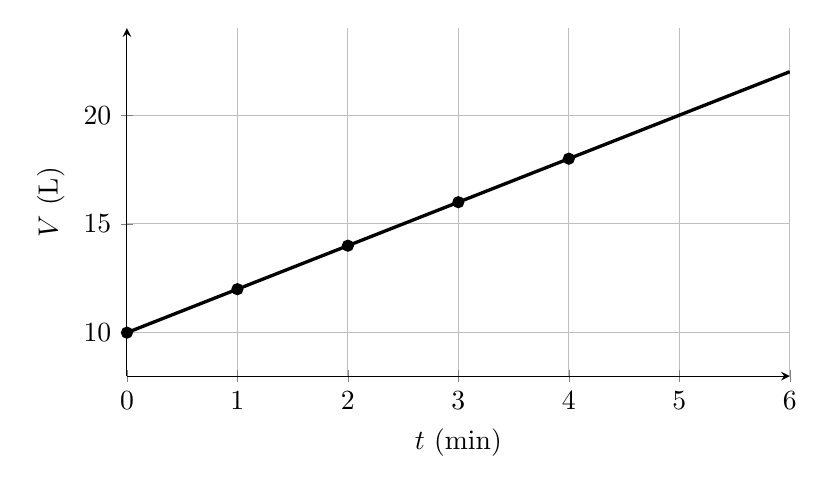
\begin{tikzpicture}
\begin{axis}[
    width=10cm,
    height=6cm,
    xmin=0,xmax=6,
    ymin=8,ymax=24,
    xlabel={$t$ (min)},
    ylabel={$V$ (L)},
    axis lines=left,
    grid=both,
    samples=100
]
\addplot[very thick,domain=0:6] {10+2*x};
\addplot[only marks,mark=*] coordinates {(0,10)(1,12)(2,14)(3,16)(4,18)};
\end{axis}
\end{tikzpicture}
\end{center}

De tabel, de grafiek en het voorschrift beschrijven dus \textbf{dezelfde relatie}.
\end{voorbeeld}

\begin{opmerking}[Een model is niet de werkelijkheid]
Een formule zoals
\[
V=10+2t
\]
is een \textbf{wiskundig model} van de situatie.

Het model is bruikbaar zolang de aannames kloppen: de instroomsnelheid blijft
constant en de tank loopt bijvoorbeeld nog niet over. Wiskunde beschrijft hier
de werkelijkheid, maar is niet de werkelijkheid zelf.
\end{opmerking}

% ------------------------------------------------------------
% STEM-voorbeeld vrije val
% ------------------------------------------------------------

\begin{voorbeeld}[Mechanica: afgelegde afstand bij vrije val]

Voor een voorwerp dat vanuit rust valt en waarbij we de luchtweerstand
verwaarlozen, gebruiken we nabij het aardoppervlak het model

\[
s(t)=\frac12 gt^2,
\]

met \(g\approx 9{,}81\ \mathrm{m/s^2}\).

Voor elke gekozen tijd \(t\) berekent het model één afgelegde afstand \(s\).

\begin{center}
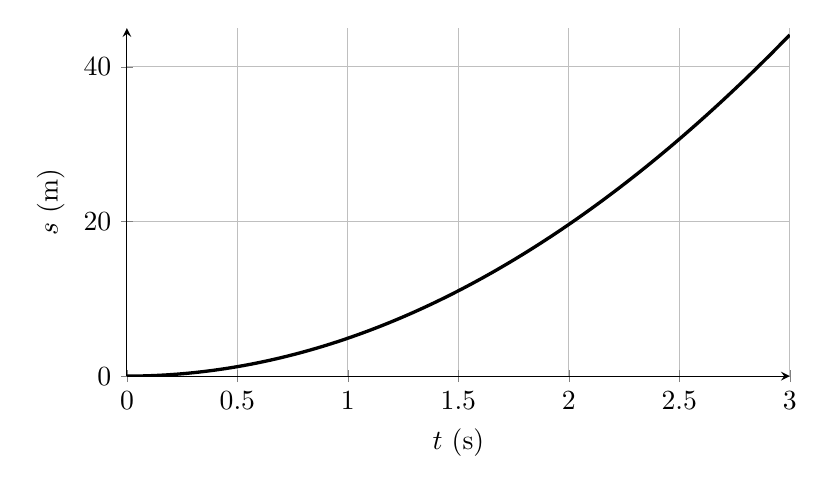
\begin{tikzpicture}
\begin{axis}[
    width=10cm,
    height=6cm,
    xmin=0,xmax=3,
    ymin=0,ymax=45,
    xlabel={$t$ (s)},
    ylabel={$s$ (m)},
    axis lines=left,
    grid=both,
    samples=150
]
\addplot[very thick,domain=0:3] {0.5*9.81*x^2};
\end{axis}
\end{tikzpicture}
\end{center}

Hoewel de formule ook voor negatieve waarden van \(t\) kan worden uitgerekend,
hebben negatieve tijden geen betekenis als \(t\) staat voor ``tijd sinds het
loslaten''. De \textbf{context} bepaalt dus mee welke waarden zinvol zijn.
\end{voorbeeld}

% ============================================================
% 2. WANNEER IS EEN RELATIE EEN FUNCTIE?
% ============================================================

\FVDsection{Wanneer is een relatie een functie?}

Niet elke relatie is een functie.

\begin{image}
    
\includegraphics{../images/Wiskunde/function_machine_1.png}
\end{image}

Het kenmerkende idee van een functie is eenvoudig maar fundamenteel:
\textbf{één toegelaten invoer mag niet tot twee verschillende uitvoerwaarden leiden}.

\begin{definitie}
Een \textbf{functie} is een relatie waarbij met iedere toegelaten invoerwaarde
\textbf{precies één} uitvoerwaarde overeenkomt.
\end{definitie}

In die definitie zijn beide woorden belangrijk:

\begin{itemize}
    \item \textbf{iedere}: een toegelaten invoerwaarde krijgt een uitvoerwaarde;
    \item \textbf{precies één}: dezelfde invoerwaarde krijgt niet twee verschillende uitvoerwaarden.
\end{itemize}

\begin{voorbeeld}[Pijldiagrammen]

Beschouw eerst de volgende afbeelding.

\begin{center}
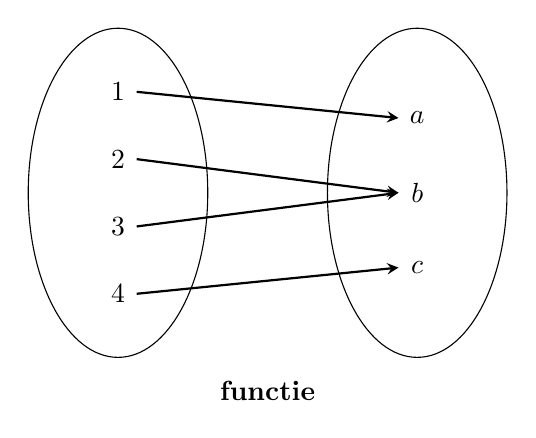
\begin{tikzpicture}[>=stealth,scale=0.95]
\draw (-2,0) ellipse (1.2 and 2.2);
\draw (2,0) ellipse (1.2 and 2.2);

\node at (-2,1.35) {$1$};
\node at (-2,0.45) {$2$};
\node at (-2,-0.45) {$3$};
\node at (-2,-1.35) {$4$};

\node at (2,1.0) {$a$};
\node at (2,0) {$b$};
\node at (2,-1.0) {$c$};

\draw[->,thick] (-1.75,1.35) -- (1.75,1.0);
\draw[->,thick] (-1.75,0.45) -- (1.75,0);
\draw[->,thick] (-1.75,-0.45) -- (1.75,0);
\draw[->,thick] (-1.75,-1.35) -- (1.75,-1.0);

\node at (0,-2.65) {\textbf{functie}};
\end{tikzpicture}
\hspace{1cm}
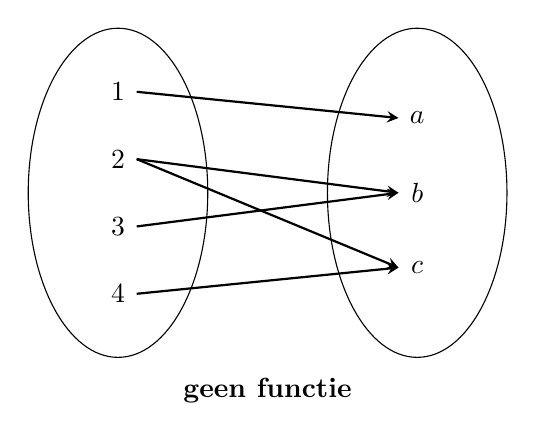
\begin{tikzpicture}[>=stealth,scale=0.95]
\draw (-2,0) ellipse (1.2 and 2.2);
\draw (2,0) ellipse (1.2 and 2.2);

\node at (-2,1.35) {$1$};
\node at (-2,0.45) {$2$};
\node at (-2,-0.45) {$3$};
\node at (-2,-1.35) {$4$};

\node at (2,1.0) {$a$};
\node at (2,0) {$b$};
\node at (2,-1.0) {$c$};

\draw[->,thick] (-1.75,1.35) -- (1.75,1.0);
\draw[->,thick] (-1.75,0.45) -- (1.75,0);
\draw[->,thick] (-1.75,0.45) -- (1.75,-1.0);
\draw[->,thick] (-1.75,-0.45) -- (1.75,0);
\draw[->,thick] (-1.75,-1.35) -- (1.75,-1.0);

\node at (0,-2.65) {\textbf{geen functie}};
\end{tikzpicture}
\end{center}

In het linker diagram vertrekt vanuit ieder element links precies één pijl.
Dat is een functie.

In het rechter diagram vertrekken vanuit \(2\) twee pijlen naar verschillende
uitvoerwaarden. Dat is geen functie.
\end{voorbeeld}

\begin{voorbeeld}[Functie of geen functie vanuit een tabel]

De tabel

\[
\begin{array}{c|cccc}
x&0&1&2&3\\
\hline
y&1&3&5&7
\end{array}
\]

beschrijft een functie: iedere gegeven \(x\)-waarde heeft precies één \(y\)-waarde.

Maar de gegevens

\[
(0,1),\quad (1,3),\quad (1,5),\quad (2,7)
\]

beschrijven \(y\) niet als functie van \(x\), want bij \(x=1\) horen
twee verschillende waarden van \(y\).
\end{voorbeeld}

\begin{opmerking}
Verschillende invoerwaarden \emph{mogen} wel dezelfde uitvoerwaarde hebben.

Bijvoorbeeld:
\[
f(-2)=4
\qquad\text{en}\qquad
f(2)=4.
\]

Dat verhindert niet dat \(f\) een functie is.
\end{opmerking}

% ============================================================
% 3. FUNCTIES GRAFISCH HERKENNEN
% ============================================================

\FVDsection{Functies grafisch herkennen}

Een grafiek bestaat uit punten \((x,y)\). Wanneer de grafiek een functie
\(y=f(x)\) voorstelt, mag bij eenzelfde \(x\)-waarde maar één \(y\)-waarde horen.

Dat leidt tot een eenvoudige grafische test.

\begin{eigenschap}[Verticale-lijntest]
Een grafiek stelt \(y\) voor als functie van \(x\) als elke verticale lijn
de grafiek in \textbf{hoogstens één punt} snijdt.
\end{eigenschap}

De verticale-lijntest is geen los trucje. Ze volgt rechtstreeks uit de definitie:
een verticale lijn kiest één vaste \(x\)-waarde. Als die lijn de grafiek op
twee verschillende hoogten snijdt, horen bij diezelfde invoer twee uitvoerwaarden.

\begin{voorbeeld}[Een parabool is een functie]

\begin{center}
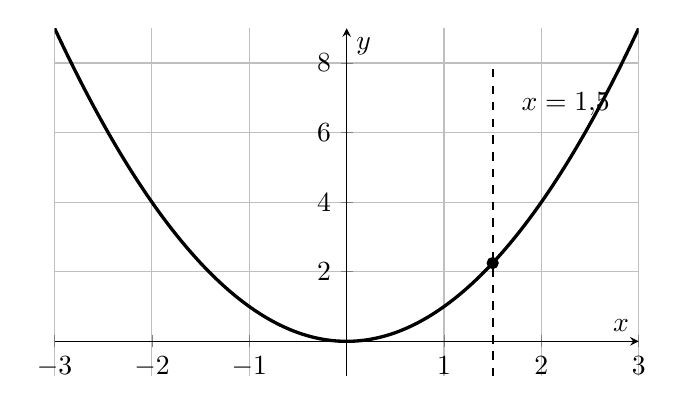
\begin{tikzpicture}
\begin{axis}[
    width=9cm,
    height=6cm,
    xmin=-3,xmax=3,
    ymin=-1,ymax=9,
    xlabel={$x$},
    ylabel={$y$},
    axis lines=middle,
    grid=both,
    samples=150
]
\addplot[very thick,domain=-3:3] {x^2};
\addplot[dashed,thick,domain=-1:8] ({1.5},x);
\addplot[only marks,mark=*] coordinates {(1.5,2.25)};
\node at (axis cs:2.25,6.8) {$x=1{,}5$};
\end{axis}
\end{tikzpicture}
\end{center}

De verticale lijn \(x=1{,}5\) snijdt de parabool één keer.
Hetzelfde geldt voor elke andere verticale lijn.
\end{voorbeeld}

\begin{voorbeeld}[Een cirkel is geen functie van \(x\)]

Beschouw de cirkel

\[
x^2+y^2=4.
\]

\begin{center}
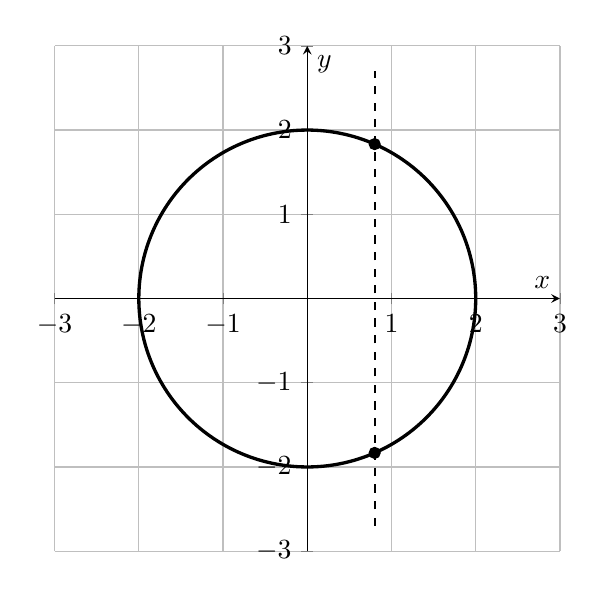
\begin{tikzpicture}
\begin{axis}[
    width=8cm,
    height=8cm,
    xmin=-3,xmax=3,
    ymin=-3,ymax=3,
    xlabel={$x$},
    ylabel={$y$},
    axis lines=middle,
    grid=both,
    axis equal image
]
\addplot[very thick,domain=0:360,samples=240] ({2*cos(x)},{2*sin(x)});
\addplot[dashed,thick,domain=-2.7:2.7] ({0.8},x);
\addplot[only marks,mark=*] coordinates {(0.8,1.833)(0.8,-1.833)};
\end{axis}
\end{tikzpicture}
\end{center}

Voor \(x=0{,}8\) vinden we twee mogelijke \(y\)-waarden:

\[
y=\pm\sqrt{4-0{,}8^2}.
\]

De verticale lijn \(x=0{,}8\) snijdt de cirkel dus tweemaal.
Daarom is \(y\) op de volledige cirkel geen functie van \(x\).
\end{voorbeeld}

\begin{fvdgeogebra}[Wanneer stelt een kromme een functie voor?]

    Open GeoGebra en teken de grafieken
    
    \[
    y=x^2,
    \qquad
    y=|x|,
    \qquad
    x^2+y^2=4,
    \qquad
    x=y^2.
    \]
    
    Maak een schuifknop \(a\) en teken de verticale lijn
    
    \[
    x=a.
    \]
    
    \begin{enumerate}
        \item Welke grafieken stellen \(y\) als functie van \(x\) voor?
        \item Wat hebben die grafieken gemeenschappelijk?
        \item Formuleer met je eigen woorden een grafisch criterium.
        \item Verklaar waarom je criterium volgt uit de definitie van een functie.
    \end{enumerate}
    
    \end{fvdgeogebra}

% ============================================================
% 4. FUNCTIENOTATIE EN FUNCTIEWAARDEN
% ============================================================

\FVDsection{Functienotatie en functiewaarden}

Een functie geven we meestal een naam, bijvoorbeeld \(f\), \(g\), \(h\) of \(T\).

Als
\[
f(x)=2x+3,
\]
dan betekent dit dat de functie \(f\) aan de invoer \(x\) de uitvoer
\(2x+3\) toekent.

We kunnen dit ook schrijven als

\[
x\longmapsto 2x+3.
\]

\begin{opmerking}[Vier dingen die je niet mag verwarren]

Bij een functie \(f\) maken we onderscheid tussen:

\[
\boxed{f}
\qquad
\boxed{x}
\qquad
\boxed{f(x)}
\qquad
\boxed{(x,f(x))}.
\]

\begin{itemize}
    \item \(f\) is de \textbf{functie};
    \item \(x\) is een \textbf{invoerwaarde};
    \item \(f(x)\) is de bijbehorende \textbf{functiewaarde};
    \item \((x,f(x))\) is een \textbf{punt op de grafiek}.
\end{itemize}
\end{opmerking}

\begin{voorbeeld}[Een functiewaarde berekenen]

Gegeven
\[
f(x)=x^2-3x+1.
\]

Dan is

\[
f(2)=2^2-3\cdot 2+1=-1.
\]

Daarom ligt het punt

\[
(2,-1)
\]

op de grafiek van \(f\).
\end{voorbeeld}

\begin{center}
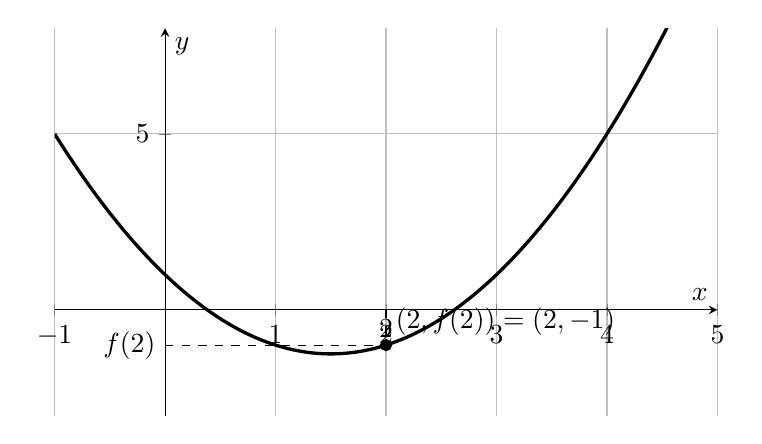
\begin{tikzpicture}
\begin{axis}[
    width=10cm,
    height=6.5cm,
    xmin=-1,xmax=5,
    ymin=-3,ymax=8,
    xlabel={$x$},
    ylabel={$y$},
    axis lines=middle,
    grid=both,
    samples=160
]
\addplot[very thick,domain=-1:5] {x^2-3*x+1};
\addplot[only marks,mark=*] coordinates {(2,-1)};
\draw[dashed] (axis cs:2,0) -- (axis cs:2,-1);
\draw[dashed] (axis cs:0,-1) -- (axis cs:2,-1);
\node[above right] at (axis cs:2,-1) {$(2,f(2))=(2,-1)$};
\node[below] at (axis cs:2,0) {$2$};
\node[left] at (axis cs:0,-1) {$f(2)$};
\end{axis}
\end{tikzpicture}
\end{center}

\begin{voorbeeld}[Interpreteren in een wetenschappelijke context]

Tijdens een eenvoudig verwarmingsproces wordt de temperatuur van een staal
gemodelleerd door

\[
T(t)=20+5t,
\]

waarbij \(t\) in minuten en \(T\) in graden Celsius wordt uitgedrukt.

Dan is

\[
T(3)=20+5\cdot3=35.
\]

Een volledig antwoord is niet alleen ``35'', maar:

\begin{center}
\emph{Volgens het model bedraagt de temperatuur na \(3\) minuten \(35^\circ\mathrm{C}\).}
\end{center}

Een berekende functiewaarde moet in een context dus opnieuw naar de
werkelijkheid worden vertaald.
\end{voorbeeld}

\begin{opmerking}
De letter tussen de haakjes hoeft niet \(x\) te zijn.

Bijvoorbeeld:

\[
h(t)=1{,}5+8t-4{,}905t^2
\]

beschrijft de hoogte \(h\) als functie van de tijd \(t\).
De notatie \(h(1)\) betekent dan: de hoogte op tijdstip \(t=1\).
\end{opmerking}

% ============================================================
% 5. ÉÉN FUNCTIE, VERSCHILLENDE VOORSTELLINGEN
% ============================================================

\FVDsection{Eén functie, verschillende voorstellingen}

Een functie kan op verschillende manieren worden voorgesteld.

\begin{center}
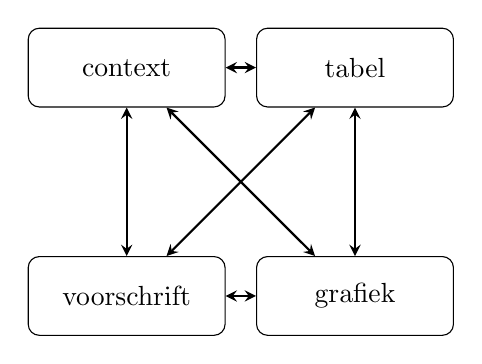
\begin{tikzpicture}[>=stealth,node distance=2.9cm]
\node[draw,rounded corners,minimum width=2.5cm,minimum height=1cm] (c) {context};
\node[draw,rounded corners,minimum width=2.5cm,minimum height=1cm,right of=c] (t) {tabel};
\node[draw,rounded corners,minimum width=2.5cm,minimum height=1cm,below of=t] (g) {grafiek};
\node[draw,rounded corners,minimum width=2.5cm,minimum height=1cm,left of=g] (v) {voorschrift};

\draw[<->,thick] (c) -- (t);
\draw[<->,thick] (t) -- (g);
\draw[<->,thick] (g) -- (v);
\draw[<->,thick] (v) -- (c);
\draw[<->,thick] (c) -- (g);
\draw[<->,thick] (t) -- (v);
\end{tikzpicture}
\end{center}

Sterk functioneren met functies betekent dat je niet vastzit aan één voorstelling.
Je moet kunnen \textbf{schakelen} tussen deze vormen.

\begin{voorbeeld}[Een rijdende robot]

Een robot rijdt langs een rechte baan. Op \(t=0\) bevindt hij zich
\(1{,}0\) meter rechts van het referentiepunt. Hij rijdt met constante snelheid
\(0{,}40\ \mathrm{m/s}\) verder naar rechts.

\textbf{Context}

\[
\text{beginpositie}=1{,}0\ \mathrm{m},
\qquad
\text{snelheid}=0{,}40\ \mathrm{m/s}.
\]

\textbf{Voorschrift}

\[
x(t)=1{,}0+0{,}40t.
\]

\textbf{Tabel}

\[
\begin{array}{c|ccccc}
t\;(\mathrm{s})&0&1&2&3&4\\
\hline
x\;(\mathrm{m})&1{,}0&1{,}4&1{,}8&2{,}2&2{,}6
\end{array}
\]

\textbf{Grafiek}

\begin{center}
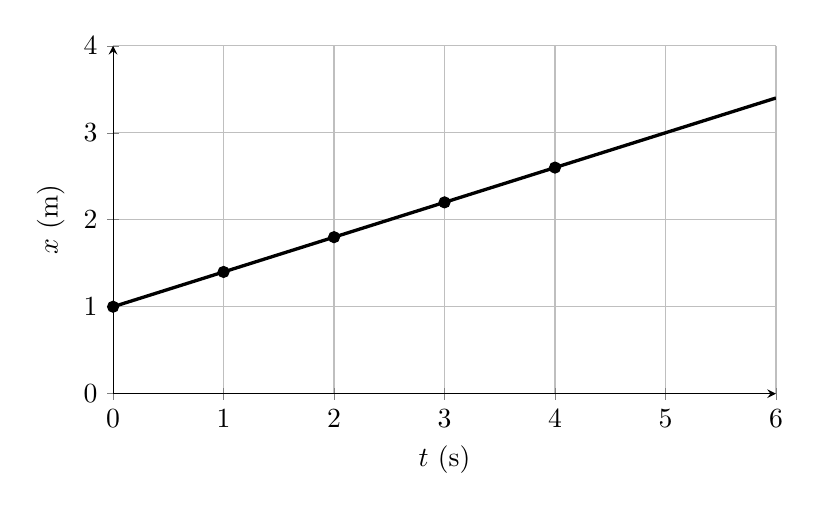
\begin{tikzpicture}
\begin{axis}[
    width=10cm,
    height=6cm,
    xmin=0,xmax=6,
    ymin=0,ymax=4,
    xlabel={$t$ (s)},
    ylabel={$x$ (m)},
    axis lines=left,
    grid=both,
    samples=100
]
\addplot[very thick,domain=0:6] {1+0.4*x};
\addplot[only marks,mark=*] coordinates {(0,1)(1,1.4)(2,1.8)(3,2.2)(4,2.6)};
\end{axis}
\end{tikzpicture}
\end{center}

Alle vier voorstellingen beschrijven hetzelfde model.
\end{voorbeeld}

\begin{fvdgeogebra}[GeoGebra als onderzoeksgereedschap]

    Gebruik GeoGebra niet alleen om een grafiek ``mooi te tekenen''.
    
    Bij een functievoorschrift kan GeoGebra helpen om:
    
    \begin{itemize}
    
        \item snel een grafiek te maken;
    
        \item punten op de grafiek te onderzoeken;
    
        \item een tabel met functiewaarden te genereren;
    
        \item vermoedens over het gedrag van de functie te formuleren;
    
        \item een grafiek met een context te vergelijken.
    
    \end{itemize}
    
    Je blijft zelf verantwoordelijk voor de interpretatie van wat GeoGebra toont.
    
    \end{fvdgeogebra}

% ============================================================
% 6. VAN WERKELIJKHEID NAAR FUNCTIE EN TERUG
% ============================================================

\FVDsection{Van werkelijkheid naar functie en terug}

Bij toepassingen doorlopen we vaak drie stappen:

\[
\boxed{\text{werkelijkheid}}
\quad\longrightarrow\quad
\boxed{\text{wiskundig model}}
\quad\longrightarrow\quad
\boxed{\text{wiskundig resultaat}}.
\]

Maar daarmee zijn we nog niet klaar. Het resultaat moet opnieuw geïnterpreteerd worden:

\[
\boxed{\text{wiskundig resultaat}}
\quad\longrightarrow\quad
\boxed{\text{betekenis in de werkelijkheid}}.
\]

\begin{voorbeeld}[Een lichtsensor]

Een eenvoudige sensor wordt in een bepaald meetbereik gekalibreerd met het model

\[
U(L)=0{,}20+0{,}015L,
\]

waarbij \(L\) de lichtsterkte in een gekozen eenheid en \(U\) de uitgangsspanning
in volt is.

Voor \(L=60\) vinden we

\[
U(60)=0{,}20+0{,}015\cdot60=1{,}10.
\]

De wiskundige uitkomst is \(1{,}10\). De interpretatie is:

\begin{center}
\emph{Volgens het model levert de sensor bij \(L=60\) een uitgangsspanning
van \(1{,}10\ \mathrm{V}\).}
\end{center}
\end{voorbeeld}

\begin{opmerking}[Kritisch denken over modellen]
Een functievoorschrift kan wiskundig voor veel waarden berekenbaar zijn,
maar dat betekent niet dat het model voor al die waarden fysisch zinvol of
betrouwbaar is.

Vraag daarom bij toepassingen steeds:

\begin{enumerate}
    \item Welke grootheden worden gekoppeld?
    \item Welke grootheid is onafhankelijk?
    \item Welke waarden zijn in de context zinvol?
    \item Wat betekent een berekende functiewaarde?
    \item Binnen welk bereik is het model geloofwaardig?
\end{enumerate}
\end{opmerking}



\end{document}
